\documentclass[a4paper]{article}
\usepackage{graphicx}
\usepackage[utf8]{inputenc}
\usepackage[english, serbian]{babel}

\title{UseCase: Registracija korisnika}
\date{10.11.2018.}

\begin{document}

\maketitle

\begin{itemize}
    \item Akter: Korisnik sistema (budući) (Glavni urednik, Urednik, Recenzent, Autor)
    \item Kratak opis: Korisnik unosi potrebne podatke kako bi se registrovao u sistemu
    \item Osnovni tok događaja:
        \begin{enumerate}
            \item Korisnik unosi podatke u formular koji mu se prikazuje nakon zahteva za registracijom (dok ne uradimo screenshot forme, ovo je placeholder formular sadrzi polja: First Name, Last Name, Title, Email, Confirm email, Password, Repeat Password, URL, Phone, Country, (check option) Available for reviewing role, Google ReCaptcha)
            \item Korisnik pokušava da se registruje
            \item Korisniku se prikazuje naredna stranica na kojoj se od njega zahteva da ulaskom na link koji mu je poslat na email, potvrdi svoj email
            \item Nakon potvrde svoje email adrese korisnik je uspešno registrovan (i ima Autorsku ulogu)
        \end{enumerate}
    \item Alternativni tok događaja:
        \begin{enumerate}
            \item Neko od obaveznih polja nije popunjeno
                \begin{enumerate}
                    \item Nakon 2. koraka sistem ispisuje poruku o grešci i zahteva od korisnika da unese podatke koji fale u obaveznim poljima i ta polja bivaju označena.
                    \item Korisnik popunjava tražena polja.
                    \item Korisnik zatim ponavlja korak 2 iz glavnog toka.
                \end{enumerate}
            \item Vrednosti u poljiva Confirm email i Repeat Password ne odgovaraju vrednostima u poljima Email i Password
                \begin{enumerate}
                    \item Nakon 2. koraka sistem ispisuje poruku o grešci i obaveštava korisnika o nepoklapanju podataka u datim poljima.
                    \item Korisnik ponovo popunjava sporna polja.
                    \item Korisnik zatim ponavlja korak 2 iz glavnog toka.
                \end{enumerate}
            \item Neko od polja ne odgovara formatu koji je za to polje zadat regularnim izrazom
                \begin{enumerate}
                    \item Nakon 2. koraka sistem ispisuje poruku o grešci i zahteva od korisnika da unese podatke u odgovarajućem formatu za polja koja označava na neki način.
                    \item Korisnik ponovo popunjava tražena polja.
                    \item Korisnik zatim ponavlja korak 2 iz glavnog toka.
                \end{enumerate}
            \item ReCaptcha ne prepoznaje korisnika kao živu osobu
                \begin{enumerate}
                    \item Nakon 1. koraka sistem ne dozvoljava korisniku da nastavi sa registracijom.
                    \item ReCaptcha se reinicijalizuje.
                    \item Korisnik ponovo pokušava da "reši"\ ReCaptcha.
                    \item Korisnik ponavlja korak c) ovog alternativnog toka 4 dok ne bude moguće preći na korak 2 glavnog toka.
                    \item Prelazi na korak 2 glavnog toka.
                \end{enumerate}
        \end{enumerate}
\end{itemize}

\begin{figure}
    \centering
    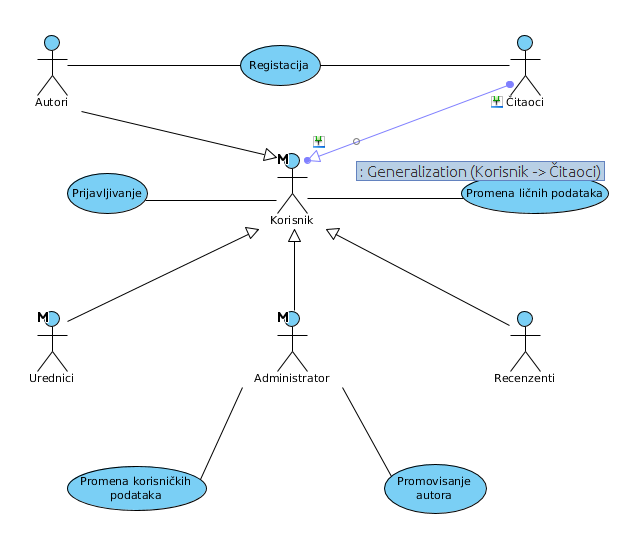
\includegraphics[width=\linewidth]{usecasePrijavljivanje.png}
    \caption{UseCase screenshot}
    \label{fig:my_label}
\end{figure}


\end{document}
